\documentclass[../CIT217_RHEL124_LabJournal.tex]{subfiles}

\begin{document}

%%%%%%%%%%%%%%%%%%%%%%%%%%%%%%%%%%%%%%%%%%%%%%%%%%%%%
%%%%%%%%%%%%%%%%%%%%%%%%%%%%%%%%%%%%%%%%%%%%%%%%%%%%%

\chapter[RHEL 124 Labs 5 \& 6]{RHEL 124\linebreak[1] Labs 5 \& 6 \hspace*{\fill}{\date}}
\noindent\textbf{{RHEL124 Labs 5 \& 6} \hspace*{\fill}{\textbf{CIT 217}}}\linebreak[1]
{{Spring 2020} \hspace*{\fill}{Chaz Davis}}                             
%===================================
%===================================
\mysection{\textbf{Chapter 5 Questions}}

\mysubsection{1}
\bf{Run the \verb$firewall-cmd --list-all$ with the necessary priviledge escalation.
Output Provided on Pg.~\pageref{ch5} See Fig~\ref{ch5}\subref{1}}
\hfill\break

\noindent\mysubsection{2}
\bf{Switch user to root. Run the command \verb$whoami$. 
Output Provided on Pg.~\pageref{ch5} See Fig~\ref{ch5}\subref{2}}
\hfill\break

\noindent\mysubsection{3}
\bf{Add your BCTC credential as a user. Change the user's password. Provide the outpupt
of the encrypted file including your user credential. 
Output Provided on Pg.~\pageref{ch5} See Fig~\ref{ch5}\subref{3}}
\hfill\break

\noindent\mysubsection{4}
\bf{Change the password policy for your user credential to require a new password every
180 days. 
Output Provided on Pg.~\pageref{ch5} See Fig~\ref{ch5}\subref{4}}
\hfill\break

\noindent\mysubsection{5}
\bf{Add a group named students with the GID of 50000. Add your user to the students
group. Provide the output of the group file including the group and your user's
membership.
Output Provided on Pg.~\pageref{ch5} See Fig~\ref{ch5}\subref{5}}

\begin{figure}[!b]\centering
	\subfloat[Output after running\\ firewall-cmd --list-all]{\label{1}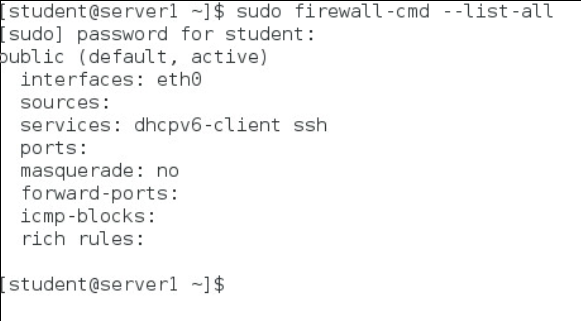
\includegraphics[width=.47\linewidth]{Figures/2020-02-06-074744_581x321_scrot.png}}\hfill
	\subfloat[Output after running whoami as
	root]{\label{2}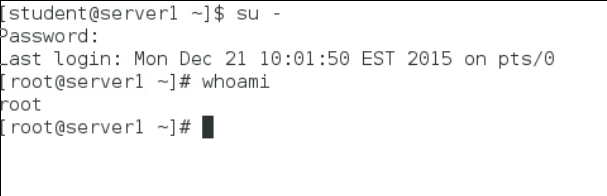
\includegraphics[width=.48\linewidth]{Figures/2020-02-06-074832_607x196_scrot.png}}\par\vspace{1.2cm} 
	\subfloat[encrypted password for my
	user]{\label{3}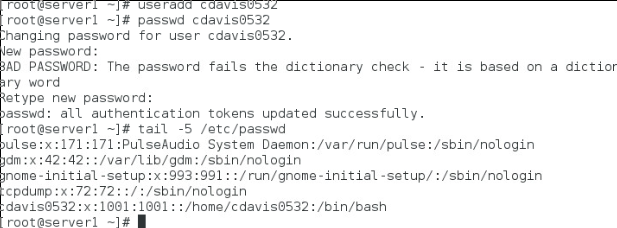
\includegraphics[width=.55\linewidth]{Figures/2020-02-06-080231_617x228_scrot.png}}\par\vspace{1.2cm}
	\subfloat[180 day password policy]{\label{4}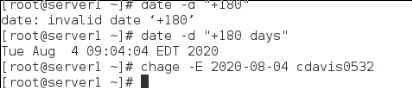
\includegraphics[width=.49\linewidth]{Figures/2020-02-06-080504_412x88_scrot.png}}\hfill
	\subfloat[Membership of the students group. with a 50000 GID]{\label{5}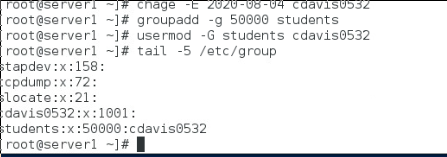
\includegraphics[width=.46\linewidth]{Figures/2020-02-06-080719_447x157_scrot.png}}\par
\caption{The Screenshots from Chapter 5}
\label{ch5}
\end{figure}


\clearpage

%===================================
\mysection{\textbf{Chapter 6 Questions}}
\mysubsection{1}
\bf{Switch user to root. Create a file named for your last name.See Fig~\ref{ch6}\subref{a} on Pg.~\pageref{ch6}. Change the permissions of the file to forbid other users from accessing it. Provide the detailed list output of the directory.  Output Provided on Pg.~\pageref{ch6} See Fig~\ref{ch6}\subref{b}}
\hfill\break

\noindent\mysubsection{2}
\bf{Add your BCTC credential as a user. Switch user to your credential. Create a file named test1. Change your umask to 027. Create a file named test2. Provide the detailed list output of the directory.  Output Provided on Pg.~\pageref{ch6} See Fig~\ref{ch6}\subref{c}}

\begin{figure}[!b]\centering
	\subfloat[Detailed list view after creating the file
	davis]{\label{a}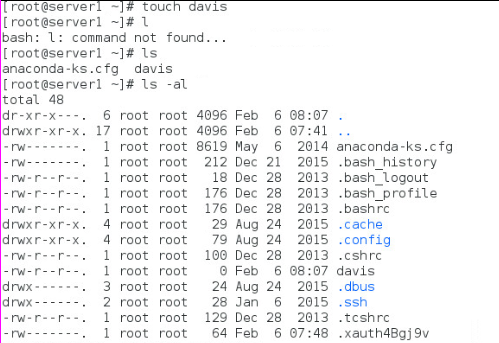
\includegraphics[width=.47\linewidth]{Figures/2020-02-06-080947_499x343_scrot.png}}\hfill
	\subfloat[Detailed List after changing file
	permissions]{\label{b}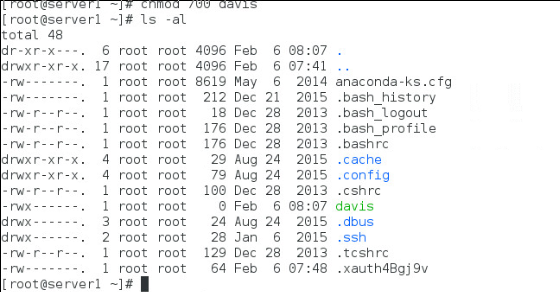
\includegraphics[width=.49\linewidth]{Figures/2020-02-06-081000_560x292_scrot.png}}\par\vspace{0.75cm} 
	\subfloat[test1 and test2 files with their umasks
	updated]{\label{c}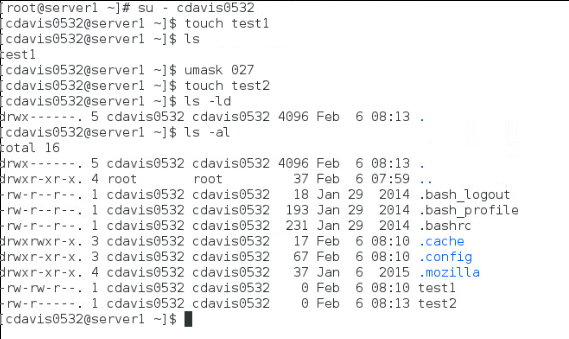
\includegraphics[width=.52\linewidth]{Figures/2020-02-06-081351_569x339_scrot.png}} 
\caption{The Screenshots from Chapter 6}
\label{ch6}
\end{figure}


%===================================
\end{document}
